%************************************************
\chapter{Hypothetical Knowledge}
\label{chapter:hypothetical_knowledge}
%************************************************

\section{Action Resources}

{\mbox{\autoref{figure:example_resource}}} shows an example of a
resource in the first-order reflective thinking layer.
\begin{figure}
\center
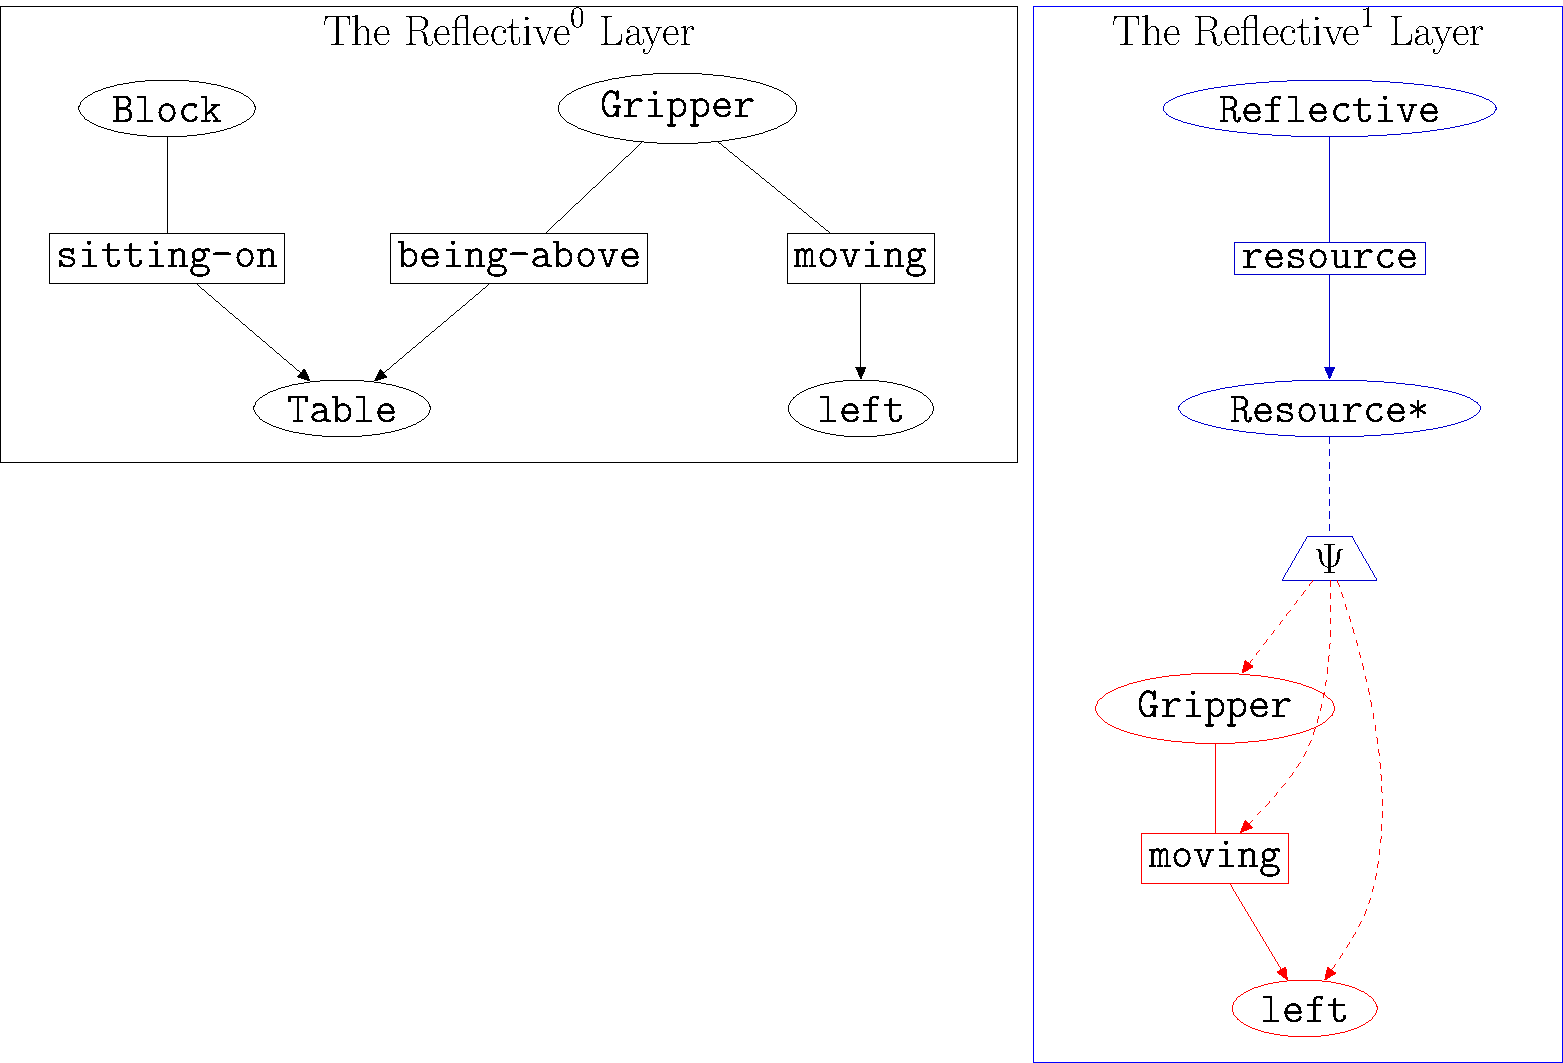
\includegraphics[width=6cm]{gfx/example_resource}
\caption{An example of a first-order reflective resource.}
\label{figure:example_resource}
\end{figure}




\section{leftovers...}

\section{Causal Knowledge}

Now that a separate temporal sequence for each reflective layer has
been defined, this factual grounded knowledge can be abstracted into
hypothetical causal models that are useful for planning toward goals
in a counterfactual future.



{\mbox{\autoref{figure:example_causal_knowledge}}} shows an example of
causal knowledge.
\begin{figure}
\center
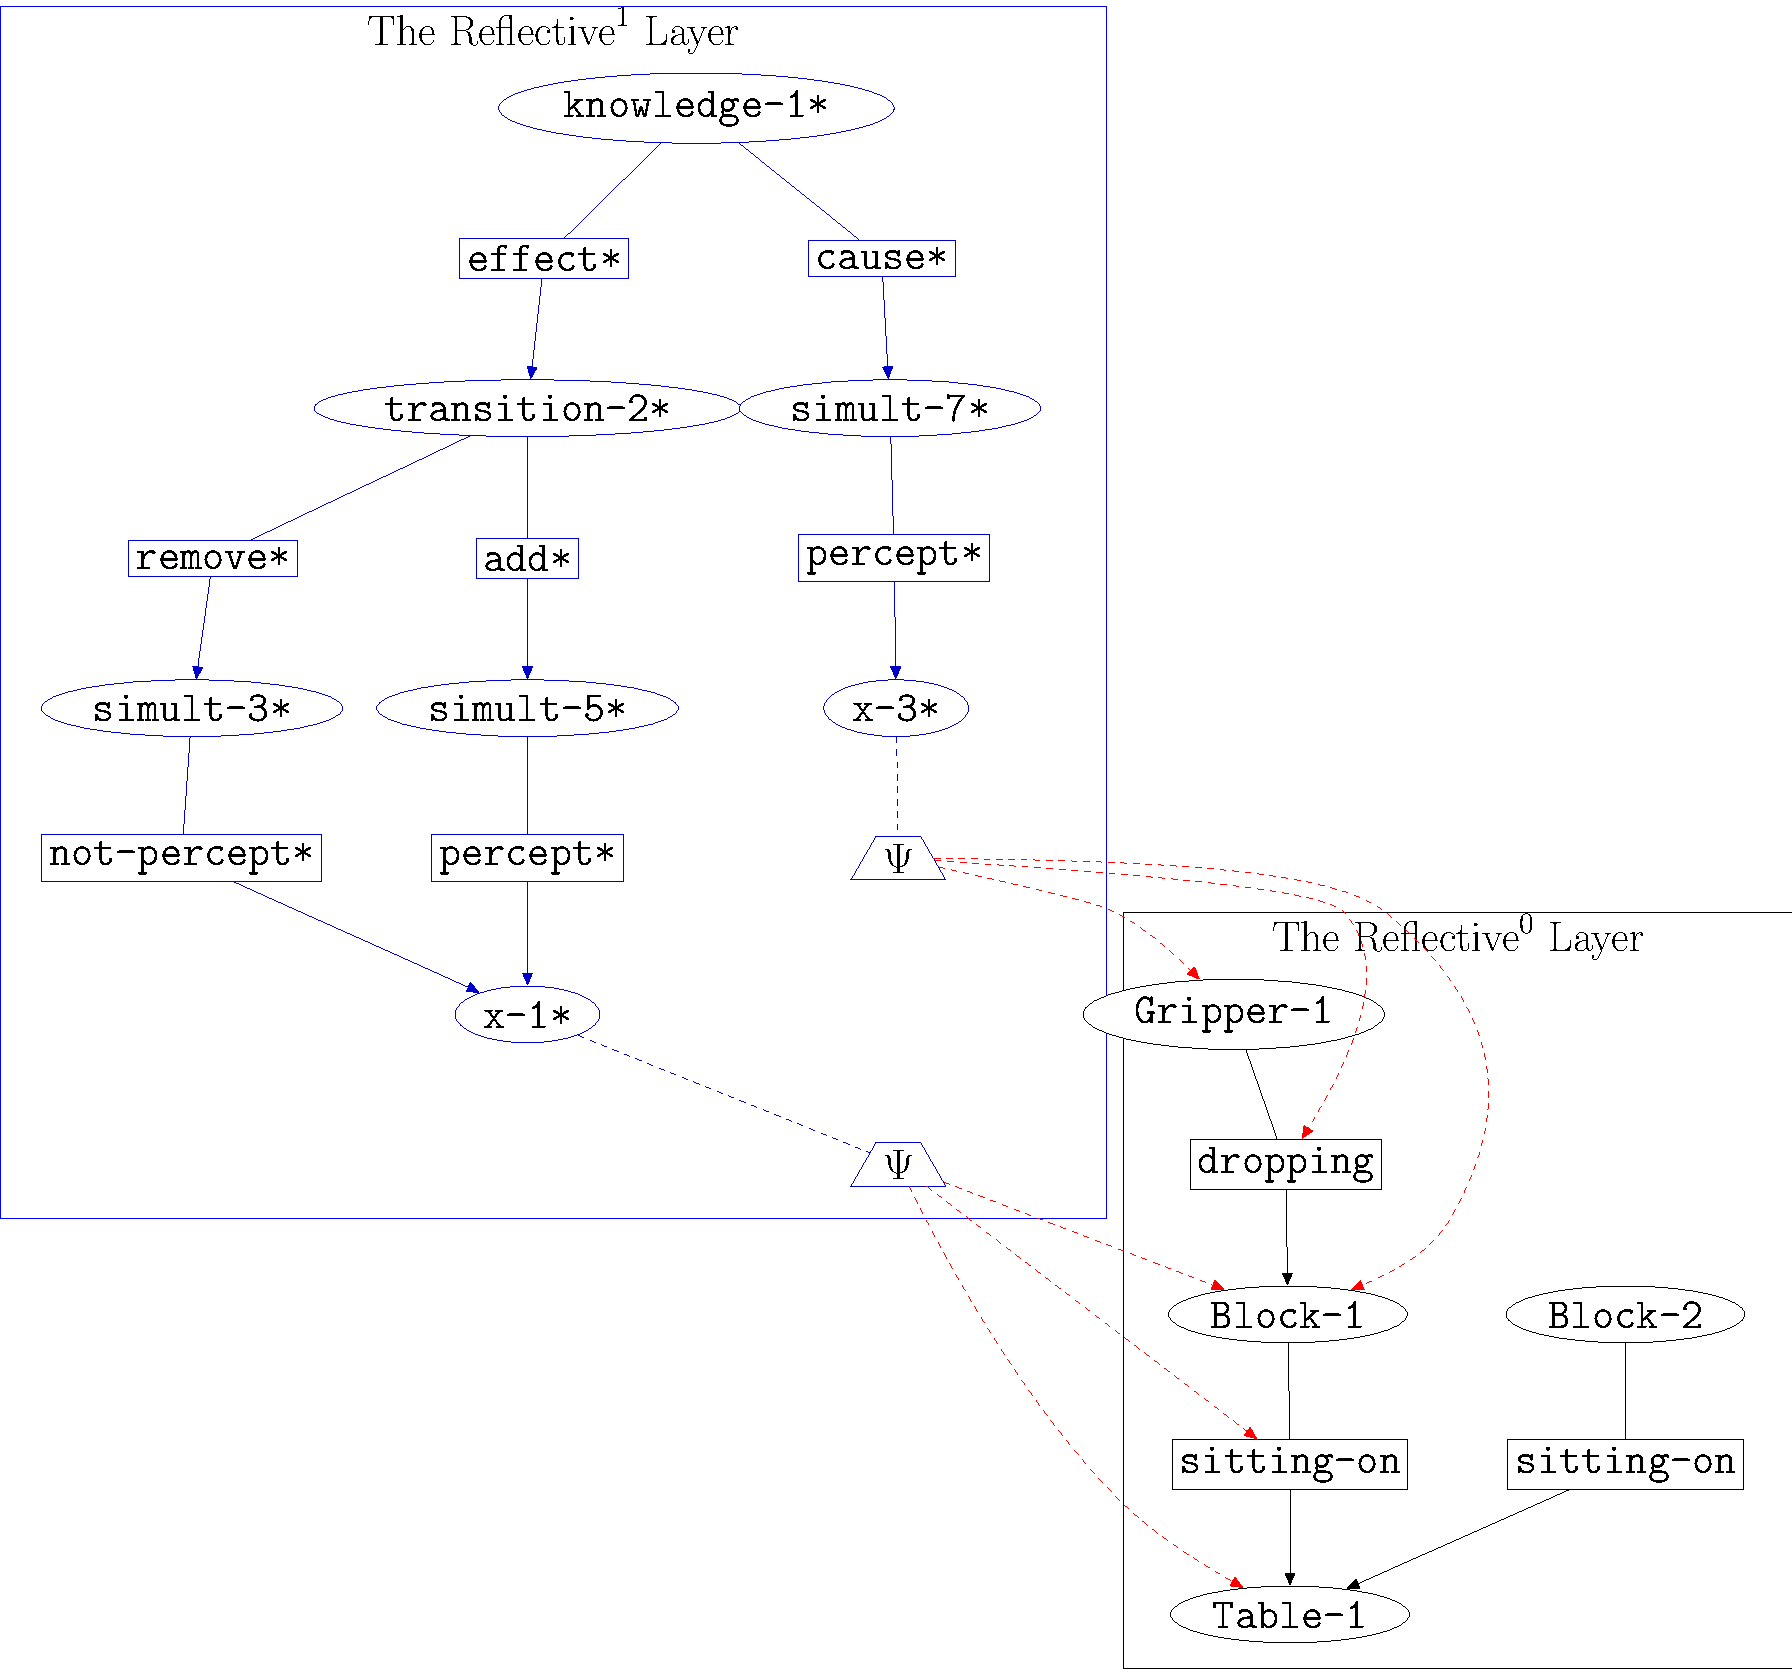
\includegraphics[width=12cm]{gfx/example_causal_knowledge}
\caption[An example of a causal knowledge.]{An example of causal
  knowledge, $\text{\tt{knowledge}}_1^*$, where the simultaneity,
  $\text{\tt{simult}}_7^*$, is known to be the cause of the
  transframe, $\text{\tt{transition}}_2^*$.  Negative perceptions are
  omitted here for to reduce visual clutter.}
\label{figure:example_causal_knowledge}
\end{figure}

\section{Representing Causal Hypotheses}

{\mbox{\autoref{figure:example_causal_hypothesis}}} shows an example
of a causal hypothesis, $h_1^*$, where the simultaneity,
$\text{\tt{simult}}_7^*$, is hypothesized to be the cause of the
transframe, $\text{\tt{transframe}}_2^*$.  In other words, the gripper
dropping the block causes the block to be sitting on the table.
\begin{figure}
\center
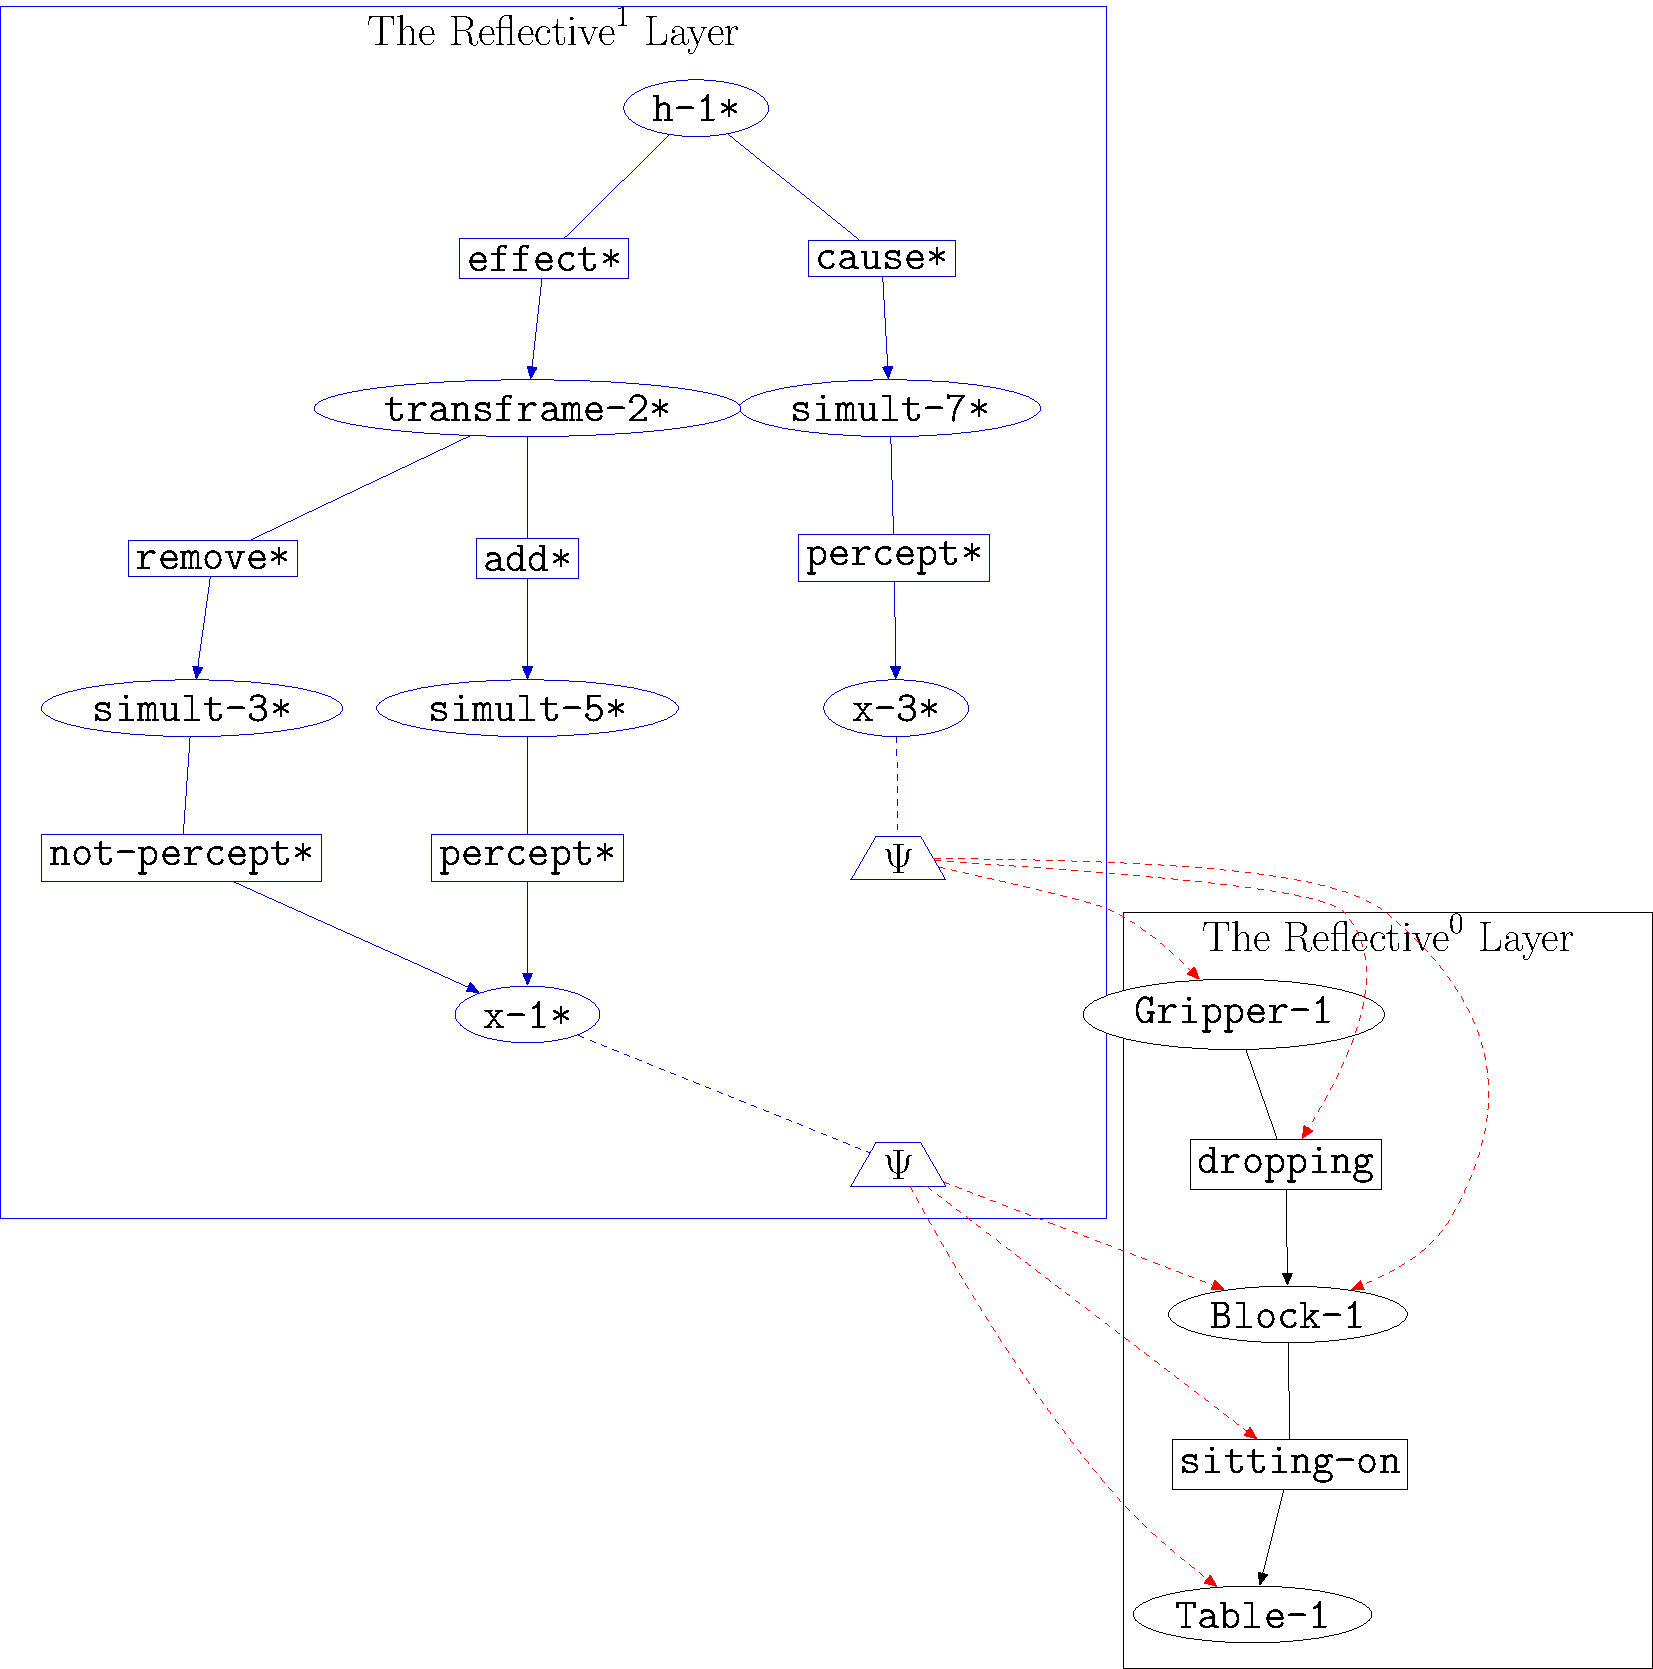
\includegraphics[width=8cm]{gfx/example_causal_hypothesis}
\caption[An example of a causal hypothesis.]{An example of a causal
  hypothesis, $h_1^*$, where the simultaneity,
  $\text{\tt{simult}}_7^*$, is hypothesized to be the cause of the
  transframe, $\text{\tt{transframe}}_2^*$.  In other words, the
  gripper dropping the block causes the block to be sitting on the
  table.}
\label{figure:example_causal_hypothesis}
\end{figure}

\section{Composing Plans from Hypotheses}

